\chapter{Instalaci\'on y explotaci\'on de quick-openstacked-hadoop}\label{cap:guiainstalacion}
\noindent Para hacer un despliegue r\'apido en un solo nodo de \texttt{qosh} y poder lanzar flujos de trabajo MapReduce sin esfuerzo, hemos habilitado un repositorio en el que se encuentran los ficheros con el c\'odigo fuente, los scripts de configuraci\'on y la imagen de la m\'aquina virtual Hadoop. Esta sencilla gu\'ia nos describe los pasos para conseguir una instalaci\'on b\'asica sin esfuerzo.

\section{Instalaci\'on r\'apida de qosh}\label{sec:instalacionqosh}

\subsection{Requisitos del sistema}\label{subsec:reqsis}
\noindent Los requisitos para que quosh se ejecute son:

\begin{itemize}
\item CPU con arquitectura x86\_64 y extensiones de virtualizaci\'on hardware (VT-x o AMD-V).
\item 4 GB de memoria RAM o m\'as.
\item 10 GB de espacio de HDD.
\item Instalaci\'on de Fedora 17.
\end{itemize}

La cantidad de memoria RAM y de espacio en disco duro van a limitar el n\'umero de instancias concurrentes que podr\'an existir ---recordemos que a cada m\'aquina virtual se le otorgan al arrancar 1 GB de RAM y 4 de HDD del anfitri\'on.

\subsection{Instalaci\'on}\label{subsec:instalacion}
\noindent La figura \ref{fig:comandosshell} contiene la serie de comandos que habr\'an de ser introducidos en un terminal para iniciar los scripts de instalaci\'on y configuraci\'on.

\begin{figure}[tbp]
 \begin{center}
  \begin{tabular}{|l|}
   \hline
   \texttt{{\bf \$} sudo yum install -y git} \\
   \texttt{{\bf \$} sudo yum update -y} \\
   \texttt{{\bf \$} sudo reboot} \\ \\
   \texttt{{\bf \$} cd <carpeta\_destino>} \\
   \texttt{{\bf \$} git clone https://code.google.com/p/quick-openstacked-hadoop} \\
   (se crear\'a la carpeta quick-openstacked-hadoop) \\ \\
   \texttt{{\bf \$} cd quick-openstacked-hadoop} \\
   \texttt{{\bf \$} sudo python install.py} \\
   (instalar\'a OpenStack Folsom, la m\'aquina virtual Hadoop, Fabric y Django) \\ \\
   \texttt{{\bf \$} python configure.py} \\
   (ajustar\'a Django) \\
   \hline
  \end{tabular}
  \caption{Serie de commandos en el terminal}
  \label{fig:comandosshell}
 \end{center}
\end{figure}

\subsection{Test de instalaci\'on}\label{subsec:testejecucion}
\noindent En este momento OpenStack y Django deber\'ian estar instalados correctamente. Para comprobar que as\'i sea abrimos la direcci\'on \url{http://localhost/dashboard} en un navegador; tras breves instantes aparecer\'a la p\'agina inicial de \texttt{Horizon} que permite iniciar sesi\'on ---el nombre de usuario por defecto es \emph{udc} y la contrase\~na \emph{udc}. Una vez introducidas las mencionadas credenciales de acceso, se nos presentar\'a la p\'agina principal para el usuario \emph{udc} en caso de que la instalaci\'on de OpenStack haya sido satisfactoria (ver imagen \ref{fig:homeos}).\newline

\begin{figure}[tbp]
\begin{center}
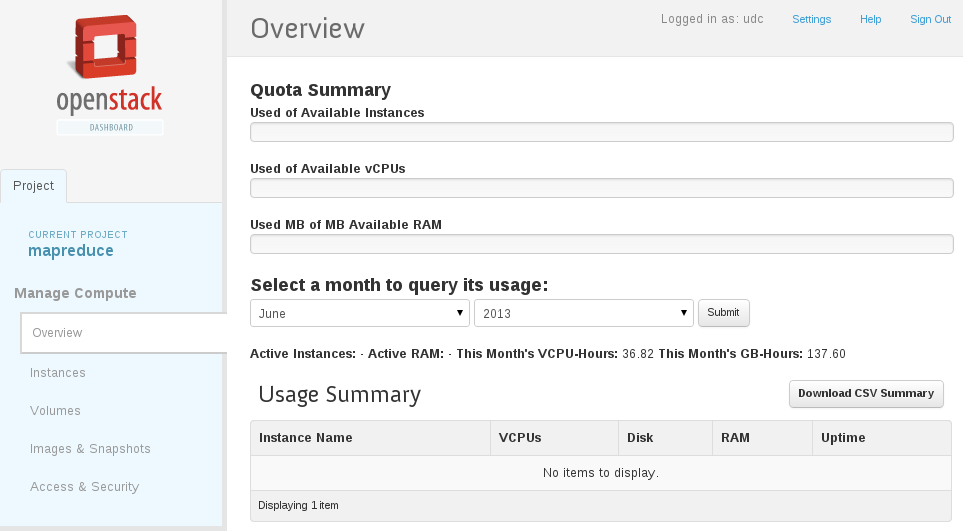
\includegraphics[width=0.99\textwidth]{imagenes/045.png}
\caption{P\'agina principal de OpenStack Folsom}
\label{fig:homeos}
\end{center}
\end{figure}

Ahora lanzaremos el servidor de desarrollo de Django para interactuar directamente con la interfaz de qosh, y as\'i comprobar su correcta configuraci\'on; la figura \ref{fig:comandosshell2} muestra la secuencia de comandos para arrancar el servidor. De nuevo, abriremos un navegador y nos dirigiremos a \url{http://localhost:8000/albaproject/mapred} para que se cargue la interfaz de acceso ---el nombre de usuario y la contrase\~na son los mismos que en OpenStack (de hecho, como se hab\'ia comentado en el cap\'itulo \ref{cap:solucion}, se delega en \texttt{Keystone} la comprobaci\'on de las credenciales de acceso a qosh).

\begin{figure}[tbp]
    \begin{center}
        \begin{tabular}{|l|}
            \hline
            \texttt{{\bf \$} cd quick-openstacked-hadoop/Alba/albaproject} \\
            \texttt{{\bf \$} python manage.py runserver} \\
            \hline
        \end{tabular}
        \caption{Serie de comandos en el terminal}
        \label{fig:comandosshell2}
    \end{center}
\end{figure}

\subsection{Flujo de prueba para Hadoop}\label{subsec:flujohadoop}
\noindent Por \'ultimo, probaremos la instalaci\'on completa haciendo el procesamiento de un trabajo MapReduce. Pueden descargarse de \url{https://code.google.com/p/quick-openstacked-hadoop/downloads/list} los ficheros que utilizaremos para la prueba de ejecuci\'on: \texttt{just\_imagine.tar.gz}, \texttt{bigtxt.tar.gz} ---ficheros comprimidos que contienen archivos de texto plano cuyo n\'umero de palabras vamos a contar--- y \texttt{wordcount.jar} ---paquete que contiene la implementaci\'on en Java del flujo MapReduce que procesar\'a Hadoop. \newline

Justo despu\'es de que nuestras credenciales hayan sido autorizadas, se carga la p\'agina principal de qosh. Desde ella haremos click en \emph{Define Job}, rellenaremos los campos del formulario de modo similar a como muestra la imagen \ref{fig:defmapredjob} y haremos click en \emph{launch} para arrancar el trabajo MapReduce. Una vez completado el procesado podremos descargar los ficheros de resultados desde la p\'agina \emph{Job History}. \newline

\begin{figure}[bp]
\begin{center}
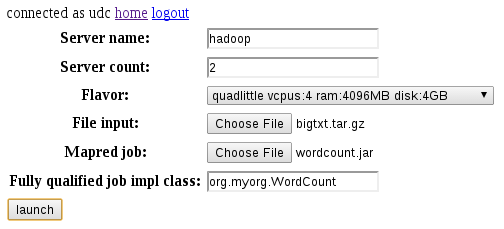
\includegraphics[width=0.90\textwidth]{imagenes/046.png}
\caption{Definici\'on de un trabajo MapReduce}
\label{fig:defmapredjob}
\end{center}
\end{figure}

La imagen \ref{fig:mapredjobhistory} muestra una captura de pantalla del historial y la imagen \ref{fig:mapredjobdetails} una captura de los detalles del trabajo n\'umero 56.


\begin{figure}[tbp]
\begin{center}
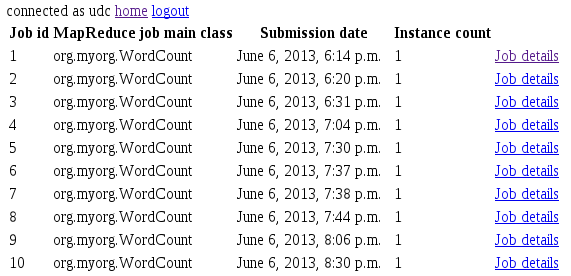
\includegraphics[width=0.99\textwidth]{imagenes/047.png}
\caption{Historial de trabajos MapReduce}
\label{fig:mapredjobhistory}
\end{center}
\end{figure}

\begin{figure}[tbp]
\begin{center}
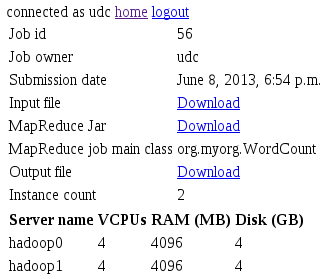
\includegraphics[width=0.60\textwidth]{imagenes/048.png}
\caption{Detalles del trabajo n\'umero 56}
\label{fig:mapredjobdetails}
\end{center}
\end{figure}


\section{Explotaci\'on y mantenimiento de qosh}\label{sec:explotacionqosh}
\noindent Para la ejecuci\'on de trabajos MapReduce de cualquier tipo habremos de seguir la operativa comentada en el apartado \ref{subsec:flujohadoop}, introduciendo cualquier paquete \emph{Jar} en el selector de fichero correspondiente y definiendo la clase principal en la caja de texto correspondiente. \newline

Como qosh se apoya en OpenStack para manejar la infraestructura, tendremos que escalar el cloud convenientemente para reducir los tiempos de latencia de trabajo ---no s\'olo es suficiente crear m\'as instancias desde la web de qosh. Para mejorar los tiempos de respuesta en la carga de p\'aginas se puede alterar el \emph{flag} \textbf{DEBUG} en el fichero \texttt{settings.py} o exportar qosh a un servidor web m\'as r\'apido. \newline

Muy brevemente, recordar que los log de OpenStack se encuentran en \texttt{/var/log/nova} y que Django hace el log siguiendo el sistema de Python 2.7. Por otra parte, resaltar que los ficheros resultado de las operaciones se encontrar\'an, por defecto, bajo \texttt{\$HOME/Public} ---esa ruta la determina la variable \textbf{MEDIA\_ROOT} en \texttt{settings.py} y puede ser alterada.




